\chapter{Artificial Neural Networks}

%\begin{comment}
\begin{wrapfigure}{r}{0.35\textwidth}
  \vspace{-20pt}
    \centering
    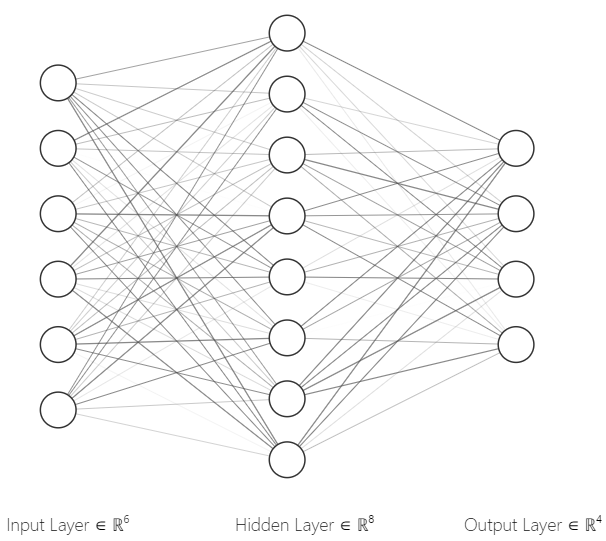
\includegraphics[width=.37\textwidth]{Figures/NN_int.png}
    \caption{\footnotesize{A two-layer neural network with the \emph{input} as the first layer and the \emph{hidden} layer as the second.  The final layer displayed is the output result}}
  \label{NNet}
  \vspace{-17pt}
\end{wrapfigure}
%\end{comment}

Inspired by the interlacing of brain tissue, artificial neural networks are what makes the extension from traditional machine learning models into deep learning methods.  Different types exist for different tasks, each with countless variations in architecture, optimization, and methods of performance measurement. A common theme to this thesis is the immense complexity of ANNs. Subject literature appears to have little to no generalizations for network types; each is a specialized or broadly encapsulative method for certain tasks.  Often, scientists of the matter seek to compare neural network features when presented with data to determine how one fairs over another when cased with similar problems. \cite{nusrat2018comparison} \cite{sharma2017activation} \cite{8371683}

ANNs are composed of one or more layers in between the input data and the output results.  Inputs propagate forward through the layers in the network, each of which performing its respective calculations toward the overall objective.  The final output is measured by a prespecified cost function (i.e. sums of squares) between the input values and desired results, and an optimization algorithm tells the network how to adjust each weight specifically in order to reduce that cost and perform better.  This chapter analyzes neural network architectures, cost functions, and  optimization algorithms; and outlines some common types of neural networks. It then reviews some techniques from modern literature on how to analyze and improve the performance of these advanced deep learning mechanisms.


%---Pathway to Architecture file---
\subfile{Architecture}  


%---Pathway to Keras_types file---
\subfile{Keras_types}

\begin{comment}
Commenting out the old text, replaced by subfile...

The previous section described a Multi-Layer Perceptron network.  This section is devoted to other network types and their most practical uses. 

Obviously not all types will be covered, but here are a few.  

%\subsection{Multi-Layer Perceptron}
%Keras Model: "sequential"
%This ws described above

\subsection{Convolutional Neural Networks}
Unstructured image data

Convolution operation // Notation // Architecture and diagram

A Convolutional Neural Network (CNN) is a neural network that uses the convolution operation in at least one of its layers \cite{?}.

Convolution operation continuous
$$
C(t) = \int x(\tau)w(t - \tau)d\tau
$$
Convolution operation discrete
$$
C(t) = \sum_{\tau = -\infty}^\infty x(\tau)w(t - \tau)
$$
$x(t)$ is the \textbf{input} and $w(t-\tau)$ is known as the \textbf{kernel}. The shorthand operation for the convolution operation is denoted with an asterisk:
$$
(x * w)(t)
$$

Assumptions for CNN's \cite{Goodfellow-et-al-2016}

\begin{itemize}
  \tightlist
  \item
output is essentially a weighted average  
 \item
$w$ must be a valid probability distribution
 \item
$w$ is 0 for all negative arguments
 \item
values of kernel and input tensors are zero except for the finite set in which values are stored (i.e. size of image)
 \item
 - infinite summation over finite number of array elements
\end{itemize}


\subsubsection{Bird Call Spectrogram example from R}

\textit{(Make brief, include Keras code, stay on track that is is simply an illustration for CNN's)}

Labeled data on recorded bird calls converted into spectrograms of 251x251 pixels.

\begin{figure}[H]
\centering
    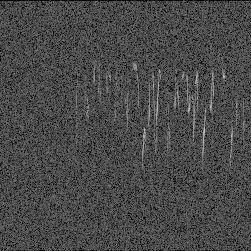
\includegraphics[width = .13\textwidth]{Figures/spectrogramsamps/Cardellina475957.png}
    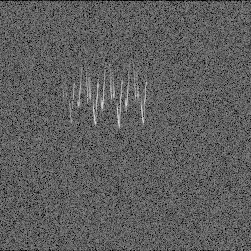
\includegraphics[width = .13\textwidth]{Figures/spectrogramsamps/Geothlypis13687.png}
    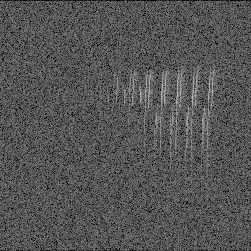
\includegraphics[width = .13\textwidth]{Figures/spectrogramsamps/Seiurus13640.png}
    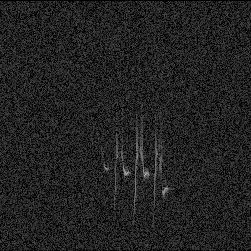
\includegraphics[width = .13\textwidth]{Figures/spectrogramsamps/Setophaga160916.png}
    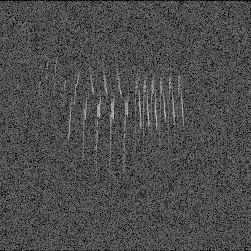
\includegraphics[width = .13\textwidth]{Figures/spectrogramsamps/Spinus192078.png}
    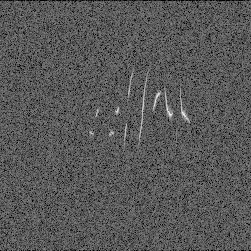
\includegraphics[width = .13\textwidth]{Figures/spectrogramsamps/Spizelloides45125.png}
    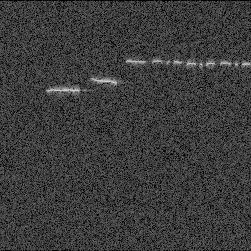
\includegraphics[width = .13\textwidth]{Figures/spectrogramsamps/Zonotrichia139053.png}
\end{figure}

Train the network to be able to identify that bird call based on spectrogram shape.

Use reference: \cite{kahl2017large}

Two-dimensional image $X$ with a two-dimensional kernel $W$
$$
C(i,j) = (X * W)(i,j) = \sum_m \sum_n X(m,n)W(i-m,j-n)
$$

$m$ and $n$ are the representative pixel locations in the relevant dimension, while $i$ and $j$ are the kernel locations, where the convolution is taking place.  The infinite summation is made possible by the fact that values are zero wherever the image is not present.



$$
Insert Example Here
$$

%---POTENTIALLY - make a pathway to the .tex file from RMarkdown ---\subfile{CNN_BCS} 


\subsection{Generative Adversarial Networks}
Unstructured image data

(Notation, no direct coding example)

Image generation to try and fool a "discriminator" network

\subsection{Recurrent Neural Networks}
Unstructured text data

(Notation, MAYBE time series coding example)

NLP/translation/text generation
Time series forecasting

\subsection{Long Short-Term Memory Network}
Unstructured text data

(Notation, no coding example)

\subsection{Convolutional Recurrent Networks}
Unstructured text data

(consider removing)

\end{comment}

\section{Techniques to Improve Model Performance} %-------------SECTION

%---Pathway to performance file---
\subfile{Performance}



\subsection{Example: Tohoku Earthquakes}

%---Pathway to earthquakes_lm_example file---
\subfile{earthquakes_lm_example}

%---Pathway to earthquakes_mlp file---
\subfile{earthquakes_mlp}

